\section{Theoretischer Hintergrund}
\subsection{Event-Driven Architecture}
\subsubsection*{Ereignisse}
Zu Beginn der Betrachtung sollte der grundlegende Begriff des Ereignisses geklärt werden. Die heute gängige Definition eines Ereignisses im Kontext von \ac*{EDA} ist, dass ein Ereignis eine 'signifikante Änderung des Zustands' ist. \cite[Vgl.][S. 4]{EDA2006} Diese relativ breite Definition hat zur Folge, dass eine große Menge an Geschäftsvorfällen als Ereignis begriffen werden kann. Als Standardbeispiel kann hier die Stornierung eines Fluges genannt werden, aber auch ein Eingang eines Auftrages, die Einstellung eines Mitarbeiters oder so etwas Reguläres wie der Beginn eines Arbeitstages, gemessen durch eine Stechuhr, konstituieren ein Ereignis. Schulte misst diesen Ereignissen in Studien für Gartner eine übergreifende Signifikanz zu. Im Grunde sei die Welt an sich ereignisgesteuert und Ereignisse als Grundlage von Architekturüberlegungen bilden diesen Umstand am besten ab. \cite[Vgl. ][S. 2]{schulte2003growing} Mit dieser Annahme als Grundlage der Betrachtung wird noch einmal die Relevanz der Überlegungen klar. Die Modellierung von Geschäftsvorfällen, oder besser Geschäftsereignissen, in einer ereignisgesteuerten Weise bildet tatsächliche Verhältnisse akkurater und intuitiver und somit besser ab, als herkömmliche Architekturansätze. \cite[Vgl. ][S. 13]{EDA2010} Diese Erkenntnis wird besonders relevant, wenn man betrachtet, dass mit einer wachsenden Gesamtmenge an Ereignissen die strukturierte Abarbeitung dieser immer wichtiger wird. Durch die immer ausgeprägteren \ac{IT} Landschaften von Unternehmen, die immer filigraner in der Lage sind Geschäftsvorfälle zu erfassen, oder Entwicklungen wie das Internet of Things, wächst die Datenmenge, die verarbeitet werden kann rapide. Die Interpretation dieser Daten als Ereignisse und deren strukturierte Verarbeitung stellt eine Möglichkeit dar, diese Daten sinnvoll zu nutzen und aus dieser Entwicklung Wert zu schöpfen. \cite[Vgl. ][S. 16]{EDA2010} 
Eine im Kontext der Unternehmenssoftware relevante Unterscheidung ist dabei die zwischen technischen und Anwendungsereignissen. Anwendungsereignisse sind Ereignisse, die fachliche Bedeutung haben, wie beispielsweise 'ein Kundenauftrag geht ein', 'eine Zahlung wurde getätigt' oder 'Ein Mitarbeiter betritt das Gebäude'. Ein technisches Ereignis hingegen ist ein Ereignis, dass ausschließlich systemintern relevant ist und zu Kommunikation und Koordination von Systemkomponenten genutzt wird. Beispiele wären 'Ein Datenbankeintrag wurde erstellt' oder 'Eine Datei wurde hochgeladen'. Es ist üblich, dass Anwendungsereignisse einen höheren semantischen Stellenwert einnehmen, also dass in der Verarbeitung eines Anwendungsereignisses viele technische Ereignisse ausgelöst werden. \cite[Vgl. ][S. 245f]{CLOUD2021}
\subsubsection*{Ereignisorientierung als Architekturansatz}
Zuerst einmal handelt es sich bei \ac{EDA}\footnote{Da sich bis jetzt keine allgemeingültige deutsche Übersetzung der Fachterminologie durchgesetzt hat, sollen in dieser Arbeit die englischen Begrifflichkeiten verwendet werden.} um ein Konzept der Prozessmodellierung. Im Gegensatz zur gewöhnlichen Ablauf-orientierten Modellierung werden die Prozesse nicht als aufeinanderfolgende Schritte, sondern als Reaktionen auf Zustände konzeptioniert. Daraus resultiert, dass nicht mehr die prozedurale Abhandlung von Arbeitsschritten die zentrale Aufgabe in der Anwendungssystem-Entwicklung darstellt, sondern die Reaktion auf Ereignisse. Im Mittelpunkt von Architekturentscheidungen steht die Frage: 'Was passiert, wenn dieses Ereignis eintritt?' und nicht mehr: 'Welche Schritte müssen zur Erfüllung dieser Anforderung gegangen werden?'. Was daraus resultiert, ist eine Architektur, die schon mit Beginn der Konzeption wesentlich agiler und robuster ist, da von Anfang an mit der Annahme gearbeitet wird, dass prinzipiell zu jedem Zeitpunkt jedes Ereignis eintreten kann. \cite[Vgl.][S.30]{EDA2010}
Ein Definitionsversuch für \ac{EDA} könnte also wie folgt lauten: Event-Driven Archtitecture bezeichnet einen Modellierungsansatz für ein verteiltes, asynchrones System, das verschiedene Komponenten durch eine zentrale Verarbeitung von Events verbindet. \cite[Vgl.][S. 248]{CLOUD2021}
\subsubsection*{Technische Grundkonzepte der \ac{EDA}}
\begin{figure}[H]
  \centering
	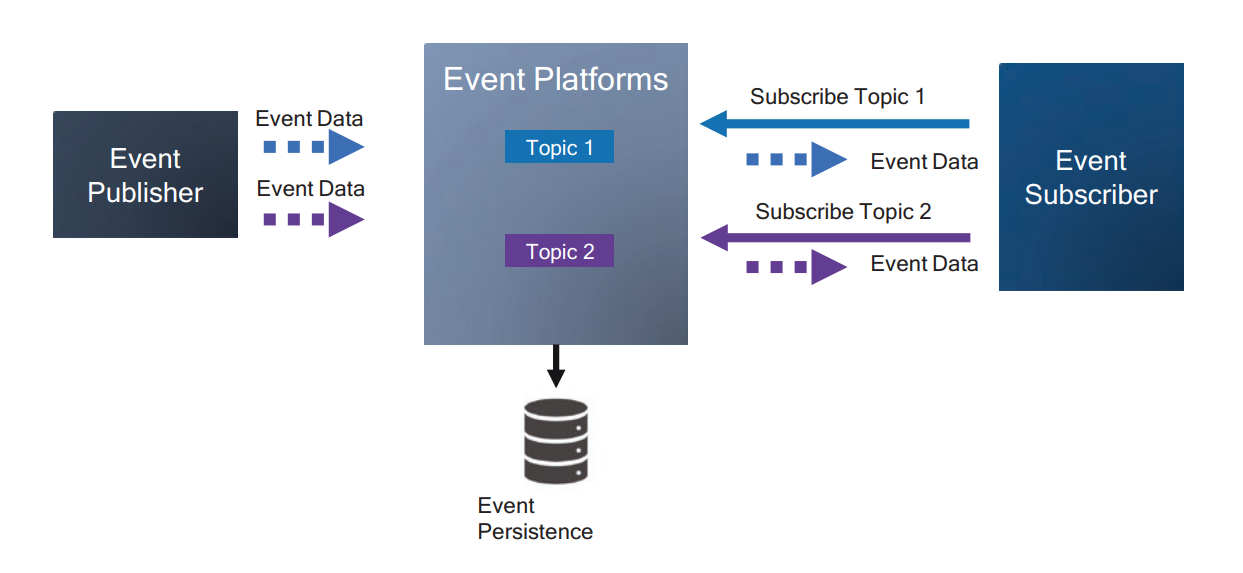
\includegraphics[width=0.8\textwidth]{Graphik EDA.png}
   \caption[Komponenten der Event-Driven Architecture]{Komponenten der \ac{EDA}\footnotemark}
\end{figure}
\footnotetext{\cite[][S. 249]{CLOUD2021}}
Die wichtigste Komponente eines durch \ac{EDA} modellierten Systems ist die zentrale Plattform zur Verarbeitung der Ereignisse in der Mitte der Architektur. Sie stellt die Infrastruktur bereit, um Events anzunehmen und diese weiterzugeben. Um einen Mehrwert aus dem System zu ziehen, muss sie darüber hinaus in der Lage sein, einen Kontext um Events herzustellen, d.h. sie in Verbindung mit anderen Ereignissen zu setzten, Ereignisse auf höheren Abstraktionsebenen zu erstellen und Ereignisse gegebenenfalls zu konsolidieren. Man spricht bei diesem Prozess von 
\ac{CEP}.\\
Weitere Komponenten des \ac{EDA} sind Publisher und Subscriber.\footnote{Für diese Komponenten finden sich in der Fachliteratur verschiedene Bezeichnungen. Außer Publisher und Subscriber findet man noch Producer und Receiver oder Producer und Listener.} Sie sind explizit von außen an das System herangeschaltet, d.h. sie haben keine Kenntnis voneinander und können auch auf völlig unterschiedlichen Plattformen basieren. Das bringt den Vorteil, dass ein durch \ac{EDA} modelliertes System inhärent modular aufgebaut ist und so zum einen weniger anfällig für Totalausfälle ist, da die Komponenten unabhängig sind, und zum anderen prädestiniert für Integrationsvorhaben ist.
Zu diesen grundlegenden Komponenten können im Zuge des \ac{CEP} noch einige weitere Konzepte hinzukommen. Die Abbildung zeigt beispielsweise eine Datenbank auf der Ereignisse persistent abgelegt werden können und die Einteilung von Ereignissen in Klassen, sogenannte Topics, die die Handhabung von verschiedenen Ereignisarten über ein System ermöglichen.\\
Hieraus ergeben sich ein paar grundlegende Fragen. Die Spezifikation der Event Platform entscheidet, wie genau Events aufgebaut sein müssen und wie Publisher und Subscriber angebunden werden. Auch weitere Überlegungen bezüglich Analyse des Ereignisflusses, Abstraktion von Ereignissen und Kompatibilität zu anderen Plattformen fallen auf Ebene der Event Platform an. Die Event Platform ist also der zentrale Baustein für die technische Umsetzung einer \ac{EDA}. \cite[Vgl. ][S. 244]{CLOUD2021}
\subsubsection*{Technische Umsetzung von \ac{EDA}}
\label{teda}
Aus den bis hierher besprochenen Grundlagen ergeben sich einige technische Überlegungen, die bei dem Aufbau einer \ac{EDA} gefasst werden müssen.

\begin{figure}[H]
  \centering
  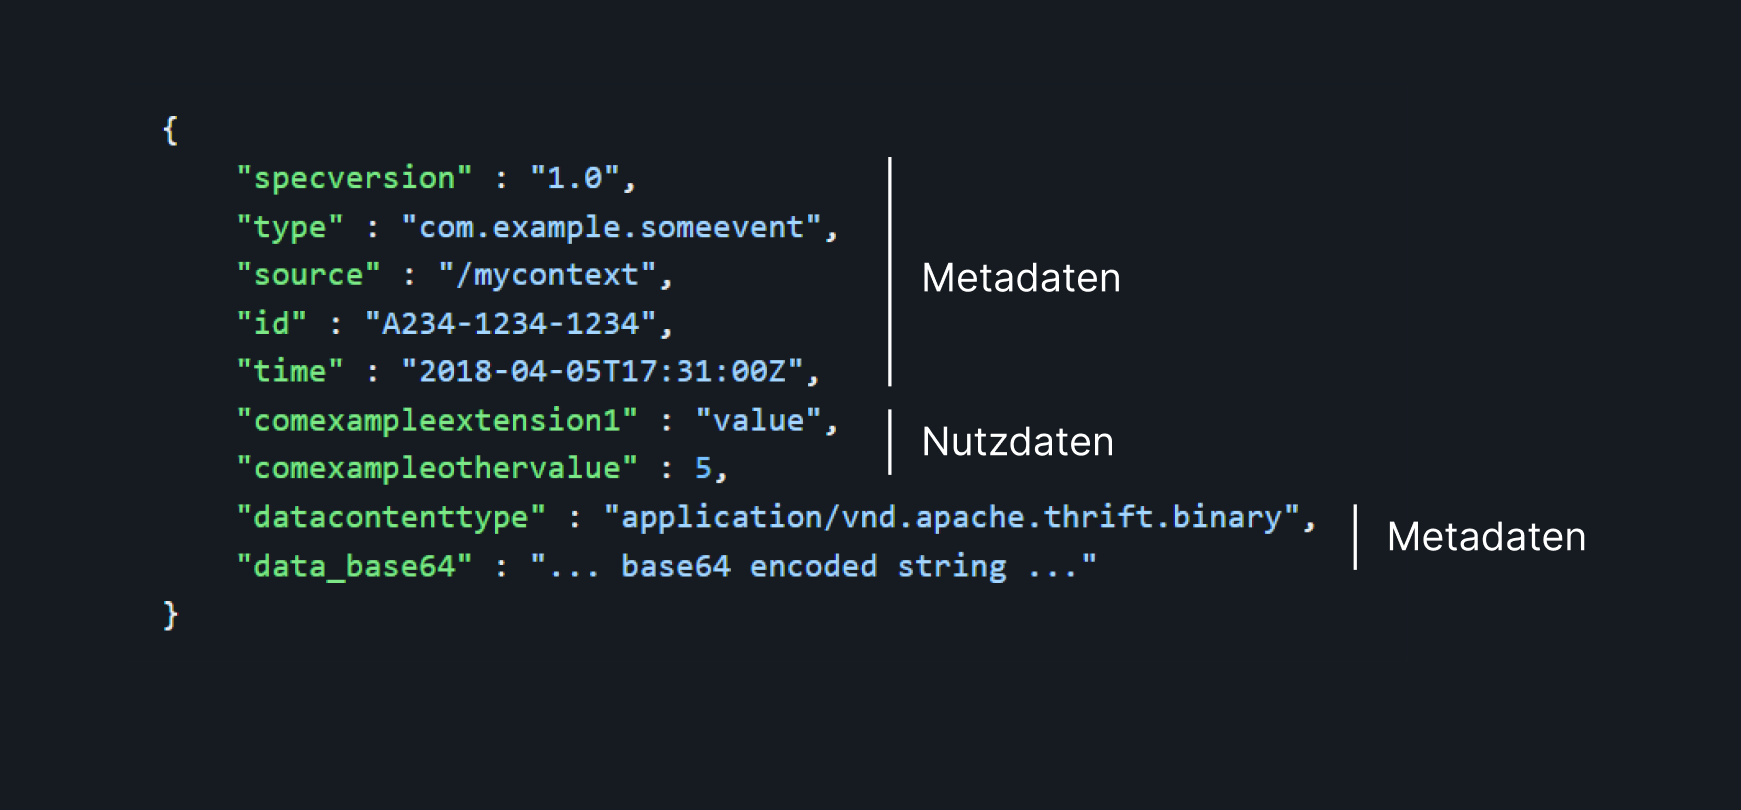
\includegraphics[width=1.0\textwidth]{Cloud Events Example.png}
  \caption[Beispiel für ein Ereignismodell]{Beispiel für ein Ereignismodell nach dem offen Standard 'CloudEvents' \footnotemark}
  \label{cloudeventslabel}
\end{figure}
\footnotetext{Eigene Darstellung nach einem Beispiel der CloudEvents Dokumentation \cite[][]{cloudeventgit}}
Ereignisse als grundlegendes Konzept der \ac{EDA} müssen in einem Ereignismodel beschrieben werden. Dieses Modell muss alle relevanten Informationen über ein Ereignis vermitteln, es sollten aber auch weitere Anforderungen an das Modell beachtet werden. Das Ereignis muss technologisch kompatibel zu allen Publishern und Subscribern sein, die an das System angeschlossen werden sollen. Es sollte zu den Nutzdaten Metadaten enthalten, die eine analytische Betrachtung des Ereignisstroms zulassen. Weiterhin sollte immer betrachtet werden, auf welcher Abstraktionsebene das Ereignis agiert, hier kann beispielsweise die technische Unterscheidung von technischen und Anwendungsereignissen sinnvoll sein. Was jedoch nie im Ereignismodell enthalten ist, ist die Verarbeitungslogik, diese liegt allein bei den Subscribern. \cite[Vgl. ][S. 95]{EDA2010} In der Anwendung werden Ereignisse häufig als strukturierter Datentyp dargestellt, JSON oder XML als Datenformat sind üblich. Ein Beispiel findet sich in Abbildung \ref{cloudeventslabel}.

Die Architektur der Event Platform hat, wie schon angerissen, besondere Relevanz. Im Grunde unterscheiden sich zwei gängige Topologien, die hier angewandt werden können: die 'Mediator-Topology' und die 'Broker-Topology'. 
\begin{figure}[H]
  \centering
  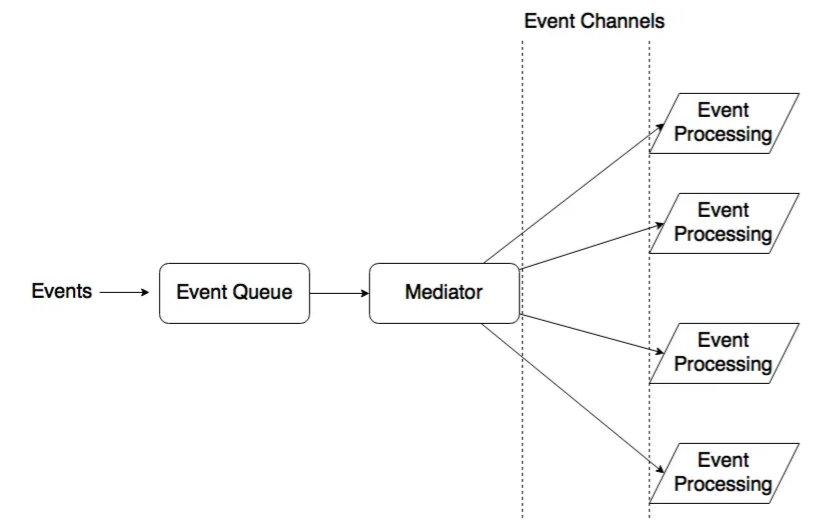
\includegraphics[width=1.0\textwidth]{Mediator Topology.png}
  \caption[Mediator-Topologie]{Mediator-Topologie \footnotemark}
  \label{mediatortop}
\end{figure}
\footnotetext{\cite[][]{wickramarachchi_2017_event}}
Die 'Mediator-Topology' sieht eine zentrale Event-Queue vor, in die Ereignisse eingespeist werden. Diese werden dann an die verschiedenen Subscriber verteilt, die anhand verschiedener Topics\footnote{In der Abbildung \ref{mediatortop} als Channels bezeichnet} gruppiert werden. Im Grunde werden in dieser Topologie also die ursprünglichen Ereignisse konsumiert und daraus folgend Ereignisse für jeden Channel, an den es gesendet werden soll, erzeugt und weitergegeben. Die Idee hinter diesem Prinzip ist es, auch Ereignisse, deren Verarbeitung mehrere Schritte benötigt orchestrieren zu können. \cite[Vgl. ][]{wickramarachchi_2017_event} \\

\begin{figure}[H]
  \centering
  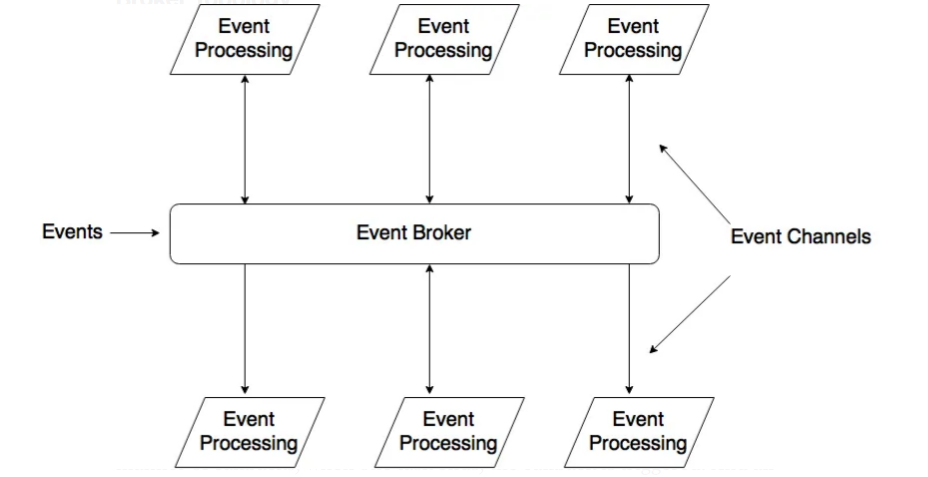
\includegraphics[width=1.0\textwidth]{Broker Topology.png}
  \caption[Broker-Topologie]{Broker-Topologie \footnotemark}
  \label{brokertop}
\end{figure}
\footnotetext{\cite[][]{wickramarachchi_2017_event}}
Die 'Broker-Topology' sieht keine zentrale Event-Queue vor. Hier werden die Ereignisse stattdessen zentral an alle relevanten Channels verteilt, ohne sie weiterzuverarbeiten. Daraus folgt, dass wenn Ereignisse mehrschrittig abgearbeitet werden müssen eine Lösung mit Callback-Ereignissen gefunden werden muss. In Abbildung \ref{brokertop} ist dies an Doppelpfeilen zu erkennen, die zwischen manchen Subscribern und dem Broker laufen. \cite[Vgl. ][]{wickramarachchi_2017_event}

\subsection{RESTful API}
\subsubsection*{API}
Martin Reddy definiert in der Einleitung seines Buch "API Design for C++" den Begriff des \ac{API} als Abstraktion eines Problems und die zugehörige Spezifikation mit der ein Anwender mit einem Software-Komponenten interagieren sollte, welcher eine Lösung für dieses Problem implementiert. \cite[Vgl. ][S. 1]{reddy2011api} Eine API ist also vordergründig eine Spezifikation, welche es ermöglicht mit Software zu interagieren. Das bedeutet sowohl, dass eine Maschine zu Maschine möglich wird, wenn die Formalisierung der Spezifikation stark genug ist, als auch, dass man nach dieser Definition eine gewöhnliche Anwendungssoftware als API, die für eine Anwender-Maschine gedacht ist, begreifen kann. Im Fachjargon der Softwareentwicklung verwendet man den Begriff der \ac{API} jedoch vordergründig, um ersteren Fall zu beschreiben. Eine praktischere Definition des Begriffes ist es also, die API als Verbindungsstück nach außen, also als Schnittstelle, einer Software-Komponente zu verstehen. \\
Eine für den Zweck der Arbeit besonders relevante Klasse von \ac{API}s sind sogenannte Web-\ac{API}s. Web-\ac{API}s sind Software-Schnittstellen, die sich das \ac{WWW} zur Nutze machen und über Protokolle des Internets angesprochen werden können. Für solche \ac{API}s haben sich über die Entwicklung des Internets eine Reihe verschiedener Standards und Architekturmuster enwtickelt, das heute eingängigste ist jedoch wahrscheinlich der REST-Standard. \cite[Vgl. ][S.5f]{richardson2007web}
\subsubsection*{REST}
Den Begriff \ac{REST} prägte erstmals Roy Fielding in seiner Dissertation im Jahr 2000. Er beschreibt damit ein Architekturprinzip für verteilte Systeme, das auf dem \ac{WWW} aufbaut. \cite[Vgl. ][S. 76]{REST2000} \ac{API}s, die dem REST Standard folgen, sogenannte \ac{REST}ful \ac{API}s, sind mittlerweile ein häufig anzutreffendes Design Muster in der Softwarearchitektur. Dabei beschreibt Fielding mit \ac{REST} an sich eigentlich kein solches Muster, sondern legt viel mehr eine Reihe von Anforderungen fest, die erfüllt sein müssen, damit eine \ac{API} \ac{REST}ful genannt werden kann. \cite[Vgl. ][S. XV]{richardson2007web} Die sechs Anforderungen, die Fielding definiert, sollen im folgenden kurz beschrieben werden:
\begin{itemize}
  \item 
  \textbf{Einheitliche Schnittstelle:} Die \ac{API} muss eine einheitliche Schnittstelle für alle Clients bereitstellen. Das bedeutet, dass alle Clients die gleichen Methoden verwenden, um mit der \ac{API} zu interagieren. Im Kontext des \ac{WWW} sind das beispielsweise die Methoden des \ac{HTTP} Protokolls.
  \item \textbf{Client-Server Architektur:} Die \ac{API} unterscheidet zwischen Client und Server, wobei diese Komponenten minimal gekoppelt sind, das heißt, im wesentlichen unabhängig in ihrer internen Funktionsweise. Client und Server kommunizieren über ein gemeinsames Protokoll, das ihre gesamte Abhängigkeit kapselt.
  \item \textbf{Zustandslosigkeit:} Die Kommunikation zwischen Client und Server ist zustandslos. Das bedeutet, dass der Server keine Informationen über den Zustand des Clients speichert und der Client bei jeder Anfrage alle Informationen, die der Server benötigt, um die Anfrage zu bearbeiten, mitgibt. 
  \item \textbf{Caching:} Die \ac{API} muss die Möglichkeit bieten, Antworten auf Anfragen zu cachen. Zur Optimierung des Diensts kann der Server also Daten mitgeben, die eine Gültigkeitsdauer haben und vom Client für diese Zeit zwischengespeichert werden können. Dadurch ist ein schnellerer Zugriff auf diese Daten möglich. Das Verfahren nennt man Caching.
  \item \textbf{Schichtensystem:} Die \ac{API} muss ein Schichtensystem unterstützen. Das bedeutet, dass der Client nicht direkt mit dem Server kommuniziert, sondern die Anfrage über eine Reihe von Zwischenstationen an den Server weitergeleitet werden kann. Diese Zwischenstationen können beispielsweise Firewalls oder Load Balancer sein.
  \item \textbf{Code on Demand:} Die \ac{API} muss die Möglichkeit bieten, Code an den Client zu senden, der dort ausgeführt wird. Das bedeutet, dass der Server nicht nur Daten an den Client sendet, sondern auch ausführbaren Code. Dieser Code kann dann beispielsweise die Darstellung der Daten übernehmen. Hierbei handelt es sich um die einzige optionale Anforderung, die Fielding definiert. \cite[Vgl. ][]{redhat_2020_was}
\end{itemize}

\subsubsection*{RESTful APIs in der Praxis des WWW}
Seit Fielding diese Anforderung im Jahr 2000 definiert hat, ist der daraus erwachsene Design-Ansatz für APIs zu einem der populärsten Muster im Entwurf von Web-APIs geworden und die rapide Entwicklung in der IT-Branche hat natürlich auch vor diesem Thema keinen Halt gemacht. In der modernen API-Entwicklung für REST spielen sogenannte Ressourcen eine entscheide Rolle, nach denen die Struktur des Dienstes modelliert wird. Eine Ressource ist dabei ein inhaltliches Element, das Gegenstand der API ist. Eine Ressource könnte beispielsweise eine Produktinformation zu einem Produkt, der Bestand eines Lagers oder die nächste Lieferung, die im Lager eintreffen soll sein. \cite[Vgl.][S. 81]{richardson2007web} Wird ein Dienst so modelliert, dass sich Anfragen an diesen immer auf solche Ressourcen beziehen, so lassen sich einfach die von Fielding definierten Anforderungen einhalten.

Man könnte sich als Beispiel eine Web API vorstellen, deren einzige Aufgabe es ist, die Temperaturdaten für eine spezifische Region zurückzugeben. Eine Ressource wäre also die Temperatur an einem bestimmten Ort zum aktuellen Zeitpunkt. Als Web API können inhärent die ersten beiden Punkte der Liste an Anforderungen abgehakt werden. Das Web legt eine Client-Server-Architektur zugrunde und die Kommunikation mit HTTP ist einheitlich. Interessant wird die Betrachtung der Zustandslosigkeit der API. Man könnte annehmen, dass das wechselnde Wetter durchaus einen Zustand darstellt und somit die REST Spezifikationen nicht mehr eingehalten werden. Die Definition gibt aber vor, dass Zustandslosigkeit nicht bedeutet, dass die API deterministisch sein muss, viel mehr wird nur verlangt, dass der Server keine Informationen über den Zustand des Clients speichert. Es darf also keine persistente Session geben, oder in anderen Worten, der Client muss mit jeder Anfrage sämtliche Informationen mitliefern, die der Server zur Verarbeitung derselben benötigt. Das ist hier durchaus der Fall. Der Client gibt mit jeder Anfrage an, für welchen Ort er die Temperatur zurückgegeben haben möchte. Das reicht dem Server aus, um die gefragte Information zurückzuliefern und er muss keine weiteren Informationen über den Zustand des Clients speichern. Weiterhin ist es in diesem Beispiel möglich die Temperaturdaten mit einem Gültigkeitszeitraum zu versehen, sodass Caching möglich wäre. Code on Demand wäre in diesem Beispiel nicht wirklich sinnvoll, ist aber auch nur optional.
\subsection{Technologie im Anwendungsbeispiel}

\subsubsection*{Cloud Events}
\label{cloudev}
Cloud Events sind ein Standard für ein Ereignismodell\footnote{Siehe Abschnitt \ref*{teda}}, um Ereignisse allgemeingültig beschreiben zu können. Von der Cloud Native Computing Foundation entwickelt, beschreibt er, wie Ereignisse aufgebaut sein müssen, um diese allgemeingültig verarbeiten und so eine Unabhängigkeit zwischen Publisher und Subscriber gewährleisten zu können. Der Standard hat mittlerweile weite Anwendung in der Industrie gefunden und wird unter anderen von Firmen wie Google, IBM und SAP in \ac{EDA}-Lösungen verwendet. \cite[Vgl. ]{cloudevent} \\
Der Standard unterstützt dabei unterschiedliche Protokolle und gibt hauptsächlich vor, welche Metadaten über das Ereignis angegeben werden müssen. So trifft er keine Aussage über die Struktur der Nutzdaten im Ereignis, sondern spezifiziert viel mehr, dass Beispielweise eine Information über den Publisher vorhanden sein muss, die Zeit und das Datum angegeben sein muss, zu der das Ereignis gesendet wurde oder eine Versionierung des Ereignisses erkennbar ist. Die Zielsetzung des Standards ist es somit nicht, inhaltliche Kompatibilität herzustellen, sondern schlicht die korrekte Verarbeitung und Weiterleitung der Ereignisse auf Seite der Event-Platform zu gewährleisten. Diese kann, da die Ereignisse, die sie verarbeitet, einem Standard folgen, Ereignisse von verschiedensten Publishern annehmen. Zudem kann, da Cloud Events für verschiedene Protokolle definiert ist, mit verschiedenen Protokollen an sie angeschlossen werden und noch mehr Unabhängigkeit geboten werden. Cloud Events selbst definiert Ziel so, "die Interoperabilität von Ereignissystemen zu definieren, die es Diensten ermöglichen, Ereignisse zu produzieren oder zu konsumieren, wobei Produzenten und Konsumenten unabhängig voneinander entwickelt und eingesetzt werden können."\ \cite[Vgl. ]{cloudeventprimer}

\subsubsection*{RAP und Business Objects}
Das \ac{RAP} ist ein Programmiermodel, das eine Reihe von Konzepten, Sprachen und Frameworks einschließt, die zusammen die Möglichkeit bieten im SAP Umfeld Applikationen unter Verwendung der Paradigmen einer \ac*{REST}ful \ac{API} zu entwickeln. \citepls

Den Kern der Entwicklung nach diesem Modell bildet die Arbeit mit sogenannten \ac{BO}s. Es handelt sich bei diesen um das Konzept von hierarchisch aufgebauten Objekten, die den Zugriff auf Daten und Aktionen, sogenannte Behaviors zu ermöglichen. An diese \ac{BO}s lassen sich zudem weitere Dienste anknüpfen, die beispielsweise die Datenstruktur in ein User-Interface umsetzen, aus ihr eine \ac{API} generieren oder Ähnliches. Ein \ac{BO} kann dabei ein beliebiges Objekt aus der echten Welt modellieren, so könnte es beispielsweise ein Produkt, eine Reise oder einen Verkaufsabschluss mit den zugehörigen Daten repräsentieren. Unter einem Hauptknoten eines solchen Objektes hängen dann weitere zugehörige Daten, aber auch Aktionen. Bei diesen kann es sich zum Beispiel um gewöhnliche transaktionale Operationen wie erstellen, löschen oder ändern handeln, aber auch dem Anwendungsfall spezifische Operationen, wie die Weiterverarbeitung eines Produktes oder die Genehmigung einer Reise sind denkbar. Um ein \ac{BO} anzulegen, werden einige Artefakte benötigt, die wichtigsten sind dabei vielleicht die Behavior Definition und die Behavior Implementation. In ersterer wird festgelegt, welche Daten und Aktion das \ac{BO} enthält, zweitere ist eine \ac{ABAP}-Klasse, deren Methoden aufgerufen werden, wenn spezifische Aktionen des \ac{BO} von der Laufzeitumgebung angefragt werden. \citepls

\subsubsection*{Business Events}
Mit Business Events können Konzepte von \ac{EDA} im SAP Umfeld umgesetzt werden. Als Business Event wird ein Ereignis bezeichnet, das durch ein Business Object im Zuge eines Behaviors erzeugt wird. Wie in Abschnitt \ref{cloudev} bereits erwähnt, folgen solche Ereignisse im SAP Umfeld dem Standard Cloud Events. Dem Ereignis werden also einige Metadaten mitgegeben, anhand derer es weiter verarbeitet wird. Der Producer eines Business Events ist also ein Business Object. 

\subsubsection*{Event Consumption Model}
\label{ecm}
Der Subscriber im SAP Umfeld ist das sogenannte Event Consumption Model. Ähnlich wie ein Business Object handelt es sich hierbei um eine Reihe von hierarchisch miteinander verknüpften Artefakten. Bereitgestellt wird beispielsweise eine \ac{ABAP}-Klasse, die die Verarbeitung des Ereignisses übernimmt, aber auch ein Service, mit dem sich der Subscriber an die Event Platform anbinden lässt. \citepls

\subsubsection*{Event Mesh}
Die Event Platform im  SAP Umfeld setzt sich aus mehreren Teilen zusammen. Der Kern ist das sogenannte Event Mesh. Dieses ist ein Dienst der \ac{BTP}, der SAP eigenen Cloud Platform. Er ist die zentrale Instanz, die die Ereignisse annimmt und weiterleitet. Er ist in der Lage, die Ereignisse zu konsolidieren, zu filtern und zu transformieren. \citepls Weiterhin sind Event Consumption Model als Subscriber und das \ac{BO} als Publisher über verschiedene Komponenten des Enterprise Event Enablement Frameworks an den Event Mesh angebunden. \citepls

\subsection{Forschungsmethodik}
\subsubsection*{Protoyping}
\label{Protoyping}
In ihrem Buch "Wirtschaftsinformatik - Einführung und Grundlegung" definieren Heinrich u.A. einen Prototypen wie folgt: "Ein Prototyp ist ein mit geringem Aufwand hergestelltes und einfach zu änderndes, ausführbares Modell des geplanten, im Entwicklungsprozess befindlichen Systems, das erprobt und beurteilt werden kann" \cite[S. 114]{heinrich2007wirtschaftsinformatik}
Als Methode zum Erkenntnisgewinn kann die Erstellung eines Prototypes also insofern eingesetzt werden, als das durch den explorativen Prozess des Erstellens des Prototypes sowohl über den Gegenstand des Prototypes, als auch über die Methode des Erstellens Erkenntnisse gewonnen werden können. Hierzu vor allem nicht nur die Erstellung des Prototyps selbst wichtig, sondern auch die strukturierte Bewertung des Prototyps im Nachgang. \cite[S. 119]{heinrich2007wirtschaftsinformatik} In dieser Arbeit soll die Erstellung es solchen Prototyps dazu verwendet werden die bis jetzt theoretisch erarbeiteten Konzepte in einem praktischen Beispiel anzuwenden und so die Erkenntnisse aus der Theorie zu vertiefen.


\subsection{Zusammenfassung des theoretischen Teils}
Ereignisse im Kontext von \ac{EDA} wurden als signifikante Änderungen des Zustands definiert. Diese Ereignisse können sowohl geschäftliche Vorfälle als auch technische Ereignisse umfassen. \ac{EDA} ist ein Ansatz zur Modellierung von Prozessen, der Ereignisse statt aufeinanderfolgender Schritte in den Vordergrund stellt. In einer \ac{EDA} stellen Publisher und Subscriber die Hauptkomponenten dar, wobei die zentrale Plattform zur Verarbeitung der Ereignisse die wichtigste Komponente ist.
RESTful \ac{API}s sind eine populäre Methode für die Gestaltung von Web-\ac{API}s. Sie folgen den Prinzipien des \ac{REST}-Architekturmodells, das von Roy Fielding definiert wurde. Dieses Modell legt eine Reihe von Anforderungen fest, die eine \ac{API} erfüllen muss, um als RESTful bezeichnet zu werden.
Weiterhin wurden verschiedene Technologien und Methoden zur Umsetzung von \ac{EDA} und RESTful \ac{API}s im SAP-Umfeld vorgestellt. Dazu gehören Cloud Events, ein Standard für Ereignismodelle, das \ac{RAP} und Business Objects zur Entwicklung von Applikationen, Business Events als Konzept für \ac{EDA} im SAP Umfeld, das Event Consumption Model als Subscriber und das Event Mesh als Event Platform.
Abschließend wurde das Konzept des Prototyping als Forschungsmethode vorgestellt, das in dieser Arbeit zur Anwendung und Vertiefung der theoretischen Erkenntnisse genutzt wird. Ein Prototyp wird dabei als ein ausführbares Modell des geplanten Systems definiert, das mit geringem Aufwand erstellt und einfach geändert werden kann.